\documentclass[a4paper]{article}
\usepackage[a4paper, left=3cm, right=2cm, top=2cm, bottom=2cm]{geometry}

\usepackage{fontspec}
\setmainfont{Times New Roman}
\usepackage{float}
\usepackage{setspace}
\singlespacing
\setlength{\parskip}{3pt}
\setlength{\parindent}{0pt}
\renewcommand{\normalsize}{\fontsize{13pt}{15.6pt}\selectfont}
\normalsize

\usepackage{tikz}
\usetikzlibrary{
	arrows.meta,
	calc,
	shapes,
	shapes.misc,
	shapes.arrows,
	chains,
	matrix,
	positioning,
	scopes,
	decorations.pathmorphing,
	shadows
}

\usepackage{cite}
\usepackage{amsmath}
\usepackage{graphicx}
\usepackage{booktabs}
\usepackage{array}
\usepackage{url}
\usepackage{listings}
\graphicspath{{./}{paper/}{paper/figures/}}
\lstdefinestyle{mystyle}{
    backgroundcolor=\color{gray!10},   
    commentstyle=\color{green!60!black},
    keywordstyle=\color{blue},
    numberstyle=\tiny\color{gray},
    stringstyle=\color{purple},
    basicstyle=\ttfamily\footnotesize,
    breaklines=true,                   % Automatically wrap long lines
    captionpos=b,                      % Caption at the bottom
    keepspaces=true,                   % Keeps spaces for indentation
    numbers=left,                      % Line numbers on the left
    numbersep=5pt,                     
    showspaces=false,                  
    showstringspaces=false,
    showtabs=false,                    
    tabsize=2
}
\lstset{style=mystyle}
\begin{document}
	
	\title{Report on the Research's Findings \\
		{\large Destructive-Read Semantics on GPU Matrix Workloads}}
	
	\author{
		Independent Interpreter Project\\
		September 2026, Hanoi}
	
	\maketitle
	
	\begin{abstract}
		\normalsize
		Sự phát triển của AI trong thời gian gần đây đã dẫn đến sự bùng nổ của nhiều thuật toán máy học và mô hình học sâu. Do vậy, nhu 
		cầu cho năng lực tính toán để học trên những bộ dữ liệu khổng lồ
		cũng từ đó tăng.
		
		Hiện nay, phép toán được sử dụng rộng rãi cho thuật toán máy học là GEMM (General Matrix Multiplication - Phép nhân ma trận tổng 
		quát). Trong quá trình học, mỗi phép nhân ma trận sẽ tạo ra một ma trận khác và ma trận mới sẽ được nối với những phép nhân ma trận khác. Để xử lý nhiều thao tác, tác vụ và quá trình khác nhau, những mô hình máy học cần thực hiện hàng triệu phép tính ma trận. Do những phép tính ma trận này so với các phép tính thông thường khác có tính đặc thù về thời gian rất cao, vì vậy những phép tính tiếp theo dần bị dồn lên bộ nhớ đệm và các bước trung gian cho đến khi những chường trình quản lý bộ nhớ hoặc quy tắc của máy tính giải phóng bộ nhớ.
		
		Việc lặp lại quá trình này đối với mô hình máy học trở thành một vấn đề lớn trong việc hoạt động dưới một khối lượng công việc rất lớn, để lại hậu quá lớn cho hiệu suất và độ trễ của mô hình trên thiết bị và tài nguyên phần cứng nó đang sử dụng.
		
		Bởi vậy, phần mềm đồng thời góp phần tối ưu hóa nhân của GEMM và tăng tuổi thọ của phần cứng được sử dụng, đảm bảo bộ đệm, dữ liệu đệm và con trỏ được giải phóng sớm nhất có thể và giảm phí tổn từ kết quả của việc dồn bộ nhớ đệm.
	\end{abstract}
	
	
	\section{Novelty}
	
	Our main goal is to directly link the precompiled \emph{cuBLAS runtime library}	 for a specific application, evaluated with a specific methodology, under an enforcement model resembling a \emph{ strictly linear type system}. Other languages have pursued related consumption-tracking semantics: Rust's ownership system~\cite{rust} enforces a comparable use-once discipline through its affine type system, and Futhark~\cite{futhark} is a purely functional array language that uses uniqueness types to support safe in-place updates. Futhark, however, generates its own GPU kernels from source rather than integrating with external, independently maintained high-performance libraries such as cuBLAS, a limitation that has been noted as one of the practical hurdles of the language. The language instead separates compile-time consumption analysis from kernel execution.
	
	\begin{equation}
		T_1 = A B,\qquad
		T_2 = T_1 C,\qquad
		T_3 = T_2 D,
	\end{equation}
	
	In implementation, numerous intermediate buffers are live at the same time. These buffers are best have their storage be erased and reused after their respective operations has run out or lifetime of the objet has ran out.
	
	Memory management benefits can be expected from a destructive-read semantics language. While arithmetic operations such as the Matrix Multiplication routine can be delegated to an optimized CUTLASS/cuBLAS kernel to circumvent \cite{futhark} Futhark's limitations. Implementation is expected to have no effect on the computational performance compared to implementation on other languages. End-end improvements, however, is expected to be present due to the optimization of the language including:
	\begin{itemize} 
		\item Reduced temporary allocation
		\item Reduced buffer lifetime
		\item Reduced GPU memory pressure
	\end{itemize}
	In theory, this implementation's effectiveness scales with the workloads, as immediate tensors or smaller matrix operations do not observe a significant impact from memory management compared to larger chained workloads.
	
	However, inherent overheads or overestimation of memory overhead or memory optimization's practicality is important to consider. Therefore, The project investigates the following hypotheses:
	
	\begin{itemize}
		\item Destructive-read semantics can reduce peak memory usage for workloads containing short-lived intermediate matrices.
		\item Destructive reads can reduce the number or cost of temporary-buffer allocations when consumed buffers can safely be reused.
		\item For workloads in which memory management represents a significant portion of total execution time, buffer reuse may improve end-to-end performance.
	\end{itemize}
	
	This project was inspired by research into destructive-read memory systems, the Sere programming language~\cite{sere}, the Clean programming language~\cite{clean}, and optimized GPU matrix-multiplication libraries.
	
	Then, Potential real-world benefits include:
	
	\begin{itemize}
		\item Improved performance for matrix multiplication operations, supporting faster training and inference for machine learning models.
		\item More effective compiler-driven reuse of intermediate tensor buffers.
		\item Reduced run-time buffer and cache allocation overhead.
	\end{itemize}
	
	\section{Background}
	
	Matrix multiplication can be written as
	
	\begin{equation}
		C_{i,j} = \sum_{k=0}^{N-1} A_{i,k}B_{k,j}
	\end{equation}
	
	Each value in the output matrix $C$ is produced by multiplying one row of $A$ with one column of $B$ and summing the products. Efficient implementations must manage data movement, memory reuse, and, in a destructive-read scheme, the lifetime of operand buffers once they are consumed.
	
	Destructive-read is a memory read operation that inherently erases the value it reads: data is destroyed at the same time it is accessed. If a value must be preserved, a write-back operation must immediately restore it, or an external buffer/cache must hold a copy.
	
	Related work on linear type systems takes a similar approach at the language level, requiring that a variable be used exactly once.
	
	Destructive-read has, historically, been more common in hardware and circuit design than in software. Dybdahl et al.~\cite{DybdahlKGN06} studied destructive-read behavior in embedded DRAM and found that removing the write-back buffer and instead relying on the cache by reading data into the cache without immediately restoring it to DRAM, and writing it back only when the cache line is replaced, offered measurable power and performance benefits. 
	
	While that result is specific to a hardware memory system, it motivates the broader question this project investigates: whether a comparable consume-on-read discipline, applied at the software/interpreter level for GEMM-heavy workloads, can yield similar results?
	
	
	\section{Project Goal}
	
	The goal of the language is to determine whether language-level destructive-read semantics can provide measurable memory-management benefits for matrix-oriented GPU programs while retaining the performance of optimized matrix multiplication kernels.
	
	The project will be implemented and evaluated through the following goals:
	
	\begin{itemize}
		\item Define language's core Python-like syntax and destructive-read semantics.
		\item Implement a lexer, parser, AST, and LLVM-based code-generation pipeline.
		\item Generate LLVM IR for arithmetic and matrix operations.
		\item Integrate optimized GPU matrix multiplication through CuBLAS.
		\item Implement explicit ownership and consumption tracking for matrix operands.
		\item Determine when consumed matrix buffers can safely be reused.
		\item Verify generated results against an independent numerical reference.
		\item Measure peak GPU memory usage and temporary-buffer allocation behavior.
		\item Measure both GPU kernel execution time and end-to-end program runtime.
		\item Compare destructive-read execution against an equivalent non-destructive implementation.
		\item Compare language against optimized GPU-library baselines where appropriate.
		\item Preserve benchmark logs, correctness results, compiler output, and build artifacts to make the experimental results reproducible.
	\end{itemize}
	
	The evaluation will not assume that destructive reads provide a performance improvement. A reduction in peak memory usage without a reduction in runtime will be treated as a meaningful result, while an observed runtime improvement will be analyzed to determine whether it originates from reduced memory-management overhead rather than from changes to the underlying matrix multiplication kernel.
	
	\subsection{Destructive-Read Semantics}
	
	A destructive read treats a value as consumed when an operation has exclusive use of that value. After consumption, the original value is no longer available to subsequent operations unless the programmer explicitly creates a copy or otherwise preserves it.
	
	For matrix operations, this provides an opportunity for storage reuse. For example,
	
	\begin{lstlisting}
		C = A @ B
		D = C @ W
	\end{lstlisting}
	
	may permit the storage associated with $A$ or $C$ to become eligible for reuse once the compiler establishes that the corresponding value has no remaining consumers.
	
	The purpose of this mechanism is not to alter the mathematical computation performed by matrix multiplication. Instead, it changes the lifetime of buffers associated with the computation. If a buffer can be reused without copying its contents, the implementation may reduce peak memory consumption and allocation activity.
	
	This optimization is inherently workload-dependent. A matrix with multiple future consumers cannot safely be destroyed after its first use. In such cases, the implementation may require a copy, borrow, or other mechanism to preserve the value. Consequently, destructive-read semantics can introduce a tradeoff between memory efficiency and the flexibility to reuse values.
	
	The language therefore treats destructive reads as an explicit ownership mechanism rather than assuming that consuming every operand will necessarily improve performance.
	
	\section{Compiler and Runtime Architecture}
	
	\subsection{ Syntax Design }
	
	We've decided on a Python-like syntax convention for the programming language:
	\begin{itemize}
		\item Comments using hashtag.
		\item Primitive Types: Integer, Float, Boolean and String.
		\item Variable declarations .
		\item Functions using 'def'.
		\item extern for runtime/FFI(cross-language) linkage.
		\item operator precendence.
		\item control flow.
	\end{itemize}
	However, due to implementation practicality and further design decision, we've decided to make adjustments to the core Python syntax:
	\begin{itemize}
		\item special precendence of clone() for cloning memory
		\item usage of braces instead of indentation for function scope
	\end{itemize}
	
	\subsection{The Free-on-Consume Scheme and cuBLAS runtime}
	The scheme referenced in \cite{DybdahlKGN06} will be used with a modified design philosophy to work at a software-level.
	\begin{table}[h]
		\centering
		\caption{Scheme implementation choices in the design}
		\label{tab:scheme-implementation}
		\begin{tabular}{ll}
			\toprule
			Dybdahl et al's DRAM & Language design \\
			\midrule
			\texttt{Data is first read from DRAM and into the cache
			} & No difference \\
			\texttt{Data are written back to DRAM when the cache line is replaced instead of if data is modified} & Operands are freed unconditionally under the assumption that the cache is always modified \\
			\texttt{Reuse the existing cache} & Uses scope-exit allocation for cache \\
			\texttt{bank interleaving ( Hide write-back by using multi-bank overlap)} & Memory free is hid behind GPU kernel launches \\
		\end{tabular}
	\end{table}

	for cuBLAS pre-compile linking:
	\begin{itemize}
		\item cuBLAS should be dynamically linked.
		\item Driver should link and ship with compiled binaries from cuBLAS.
		\item For convenience, distributed as a packaged file.
	\end{itemize}

	
	\section{File structure}
	
	\subsection{ Pipeline } 
	\begin{figure}[H]
		\centering
		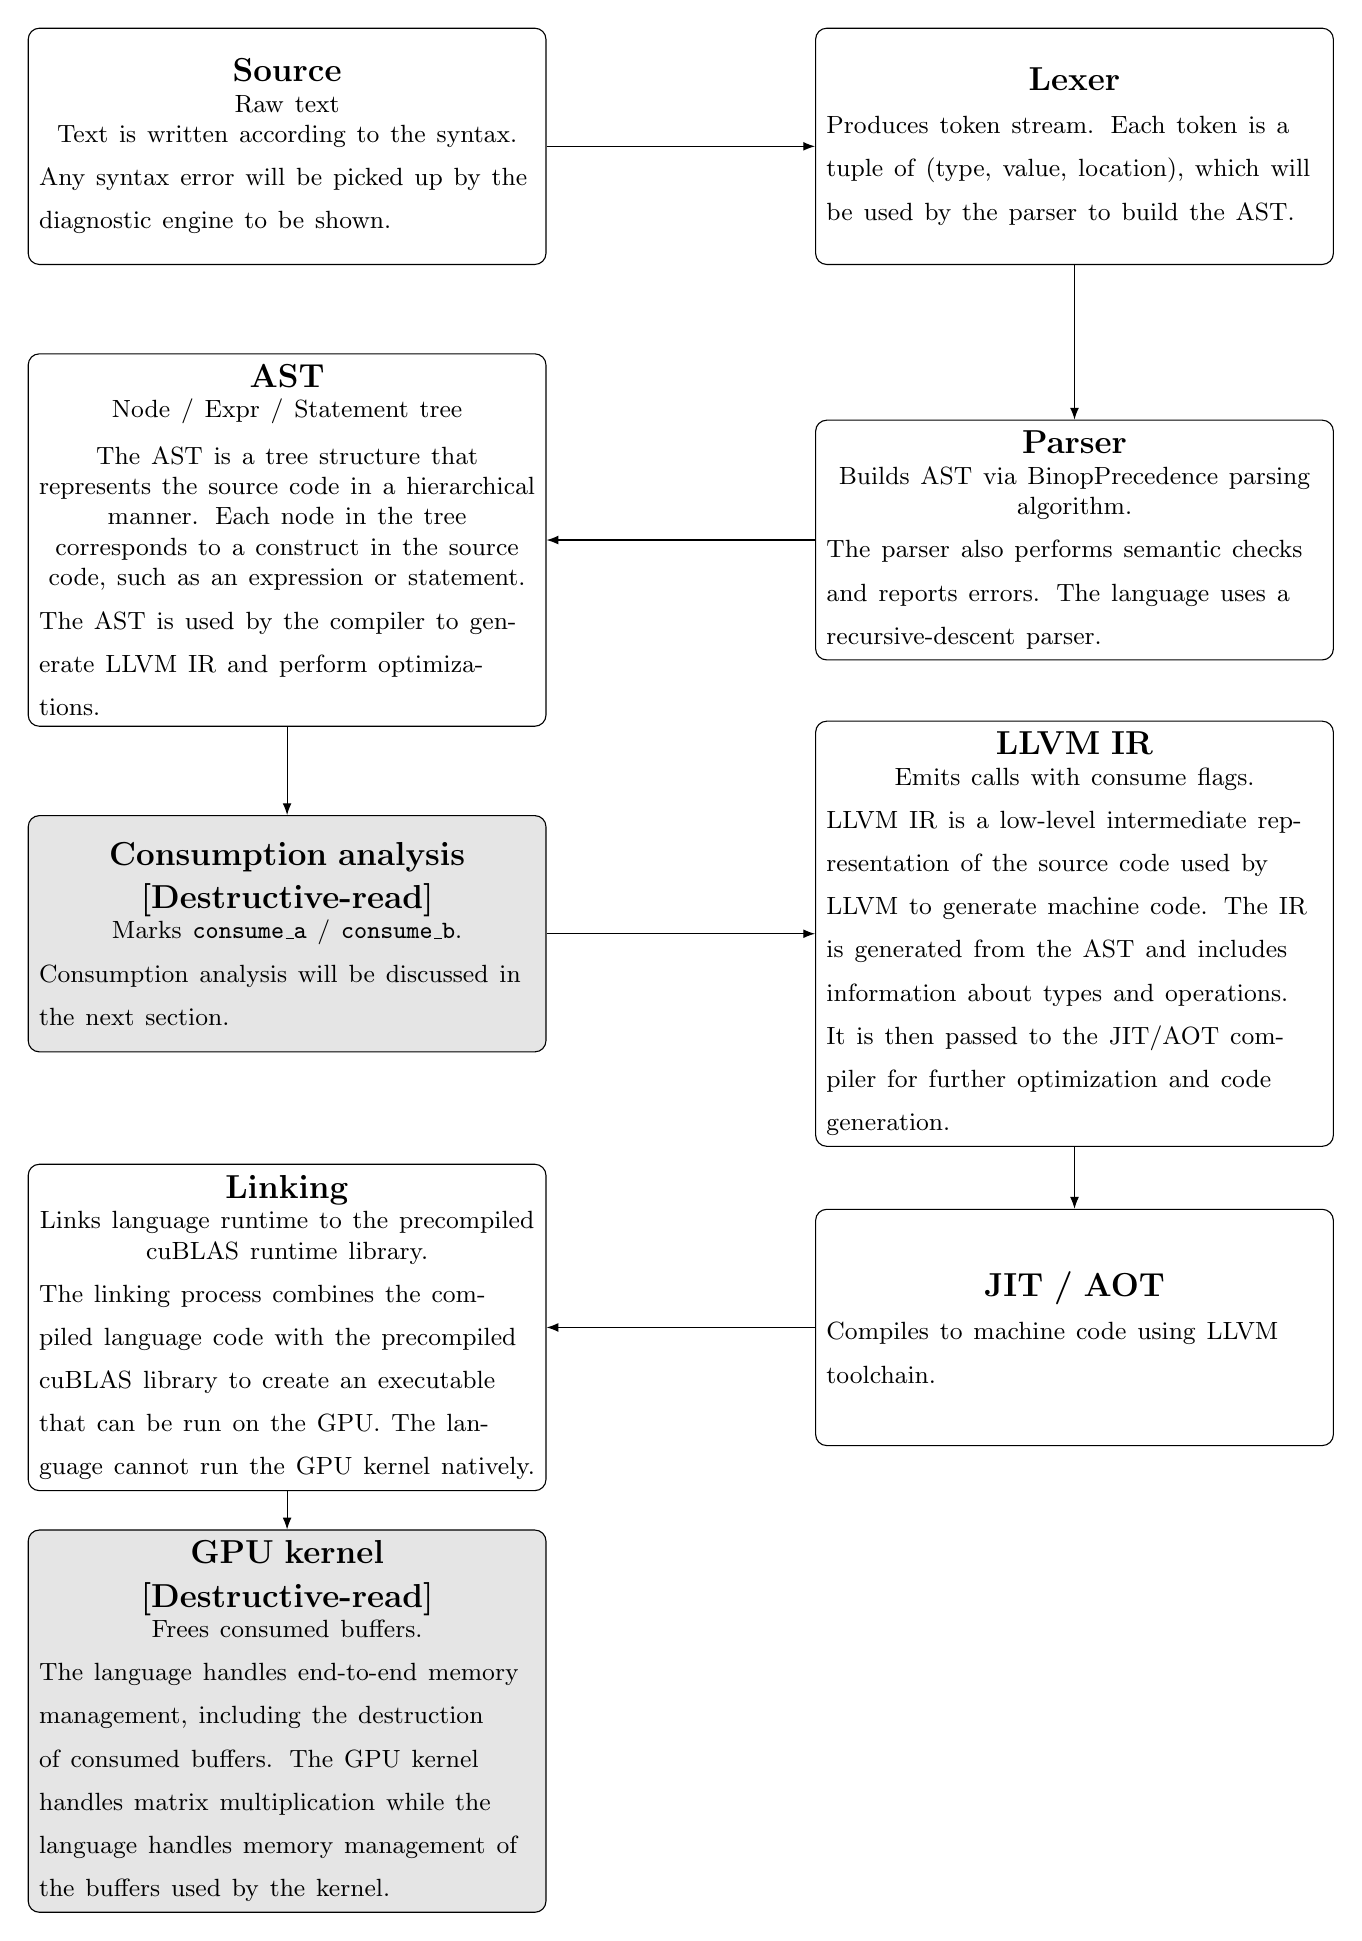
\begin{tikzpicture}[
			node distance=5cm,
			box/.style={
				rectangle,
				draw,
				rounded corners,
				minimum width=6.3cm,
				text width=6.3cm,
				minimum height=3cm,
				align=left,
				font=\normalsize
			},
			special/.style={
				box,
				fill=gray!20
			},
			arr/.style={
				-{Latex[length=1.5mm]}
			}
			]
			
			\node[box] (src) at (0,0) {
				\centering\textbf{Source}\\
				\small Raw text\\
				Text is written according to the syntax.\\
				\small Any syntax error will be picked up by the diagnostic engine to be shown.
			};
			
			\node[box] (lex) at (10,0) {
				\centering\textbf{Lexer}\\
				\small Produces token stream. Each token is a tuple of
				(type, value, location), which will be used by the parser
				to build the AST.
			};
			
			\node[box] (par) at (10,-5) {
				\centering\textbf{Parser}\\
				\small Builds AST via BinopPrecedence parsing algorithm.\\
				\small The parser also performs semantic checks and reports errors.
				The language uses a recursive-descent parser.
			};
			
			\node[box] (ast) at (0,-5) {
				\centering\textbf{AST}\\
				\small Node / Expr / Statement tree\\[2mm]
				\small The AST is a tree structure that represents the source code
				in a hierarchical manner. Each node in the tree corresponds to a
				construct in the source code, such as an expression or statement.\\
				\small The AST is used by the compiler to generate LLVM IR and
				perform optimizations.
			};
			
			\node[special] (con) at (0,-10) {
				\centering\textbf{Consumption analysis [Destructive-read]}\\
				\small Marks \texttt{consume\_a} / \texttt{consume\_b}.\\
				\small Consumption analysis will be discussed in the next section.
			};
			
			\node[box] (ir) at (10,-10) {
				\centering\textbf{LLVM IR}\\
				\small Emits calls with consume flags.\\
				\small LLVM IR is a low-level intermediate representation of the
				source code used by LLVM to generate machine code. The IR is
				generated from the AST and includes information about types and
				operations. It is then passed to the JIT/AOT compiler for further
				optimization and code generation.
			};
			
			\node[box] (jit) at (10,-15) {
				\centering\textbf{JIT / AOT}\\
				\small Compiles to machine code using LLVM toolchain.
			};
			
			\node[box] (link) at (0,-15) {
				\centering\textbf{Linking}\\
				\small Links language runtime to the precompiled cuBLAS runtime
				library.\\
				\small The linking process combines the compiled language code
				with the precompiled cuBLAS library to create an executable that
				can be run on the GPU. The language cannot run the GPU kernel
				natively.
			};
			
			\node[special] (gpu) at (0,-20) {
				\centering\textbf{GPU kernel [Destructive-read]}\\
				\small Frees consumed buffers.\\
				\small The language handles end-to-end memory management,
				including the destruction of consumed buffers. The GPU kernel
				handles matrix multiplication while the language handles memory
				management of the buffers used by the kernel.
			};
			
			\draw[arr] (src) -- (lex);
			\draw[arr] (lex) -- (par);
			\draw[arr] (par) -- (ast);
			\draw[arr] (ast) -- (con);
			\draw[arr] (con) -- (ir);
			\draw[arr] (ir) -- (jit);
			\draw[arr] (jit) -- (link);
			\draw[arr] (link) -- (gpu);
			
		\end{tikzpicture}
		
		\caption{The memory pipeline, which encompasses the process from source text to GPU execution. Shaded figures denote where destructive-read semantics are relevant.}
		\label{fig:pipeline}
	\end{figure}

	\begin{table}[h]
		\centering
		\caption{Main Source Files}
		\label{tab:modules}
		\begin{tabular}{ll}
			\toprule
			File & Purpose \\
			\midrule
			\texttt{Lexer.h/.cpp} & Tokenizes language source \\
			\texttt{Parser.h/.cpp} & Builds the AST \\
			\texttt{ExprAST.h} & AST node definitions \\
			\texttt{CodeGen.cpp} & LLVM IR generation \\
			\texttt{CuBLASRuntime.cpp} & cuBLAS MatMul bindings \\
			\texttt{main.cpp} & Driver / REPL \\
			\bottomrule
		\end{tabular}
	\end{table}
	
	\section{Verification}
	
	
	\begin{table}[h]
		\centering
		\caption{Correctness Test Results}
		\label{tab:verification}
		\begin{tabular}{ll}
			\toprule
			Test Case & Result \\
			\midrule
			$N \times N$ MatMul vs. reference (conventional) & TBD \\
			Destructive-read re-use error detection (runtime) & TBD \\
			Edge cases (empty, 1x1, non-square) & TBD \\
			\bottomrule
		\end{tabular}
	\end{table}

	$N \times $N MatMul vs. reference (conventional): Evaluating a chain of matrix multiplication operations to stress-test for evaluating end-to-end improvements.
	Destructive-read re-use errordetection: Evaluates at run and compile time to sort for errors 
	Edge cases: Evaluate edgecases to stress test compatability and thoroughness of the algorithm.
	
	
	\section{Benchmarks}
	
	The benchmark evaluation is designed to distinguish improvements in memory management from improvements in matrix multiplication itself.
	
	Three primary implementations will be compared:
	
	\begin{enumerate}
		\item An optimized GPU-library implementation used as a kernel-performance reference.
		\item language using conventional non-destructive value semantics.
		\item language using destructive-read semantics.
	\end{enumerate}
	
	Where appropriate, a simple C++ or CUDA implementation will also be included as a baseline.
	
	The most important comparison is between the two languages configurations. Both configurations perform the same mathematical operations and use the same underlying GPU matrix multiplication implementation. This comparison isolates the effect of destructive-read semantics more effectively than a comparison against an unrelated implementation.
	
	The benchmark suite will include isolated matrix multiplications as well as chains of matrix operations. Matrix dimensions will include small, medium, large, and non-square matrices. This allows the evaluation to determine whether the effect of destructive reads depends on workload size.
	
	The following measurements will be collected:
	
	\begin{itemize}
		\item GPU kernel execution time.
		\item End-to-end execution time.
		\item Peak GPU memory consumption.
		\item Number of temporary-buffer allocations.
		\item Number of buffer reuse events.
		\item Host-to-device and device-to-host transfer time where applicable.
		\item Compiler and runtime overhead.
		\item Numerical error relative to a reference implementation.
		\item GPU power draw.
	\end{itemize}
	
	GPU measurements will use multiple repetitions and appropriate warm-up iterations. CUDA initialization and compilation overhead will be separated from steady-state execution measurements where possible.
	
	The benchmark will report both absolute measurements and relative changes. No performance improvement will be attributed to destructive-read semantics unless the corresponding measurements support that interpretation.
	
	
	
	\subsection{Expected Relationship Between Language and MatMul Performance}
	
	The expected execution time can be approximately decomposed as
	
	\begin{equation}
		T_{\mathrm{total}} =
		T_{\mathrm{language}} +
		T_{\mathrm{memory}} +
		T_{\mathrm{launch}} +
		T_{\mathrm{kernel}}.
	\end{equation}
	
	Destructive-read semantics primarily target $T_{\mathrm{memory}}$. They are not expected to substantially reduce $T_{\mathrm{kernel}}$ when the same optimized GPU kernel is used.
	
	For a large matrix multiplication, $T_{\mathrm{kernel}}$ may dominate the total execution time, resulting in little observable end-to-end improvement. For workloads containing many intermediate tensors or small matrix operations, however, $T_{\mathrm{memory}}$ and other runtime costs may become more significant. 
	
	
	
	
	\section{Evidence and Reproducibility}
	\label{sec:evidence}
	
	Add an example build here: 
	\begin{lstlisting}[caption = Example compilation]
	def basicadd(int i, int k) {
		return i + k;
		}
	# Basic compilation of source code, addition only. No showcase of GEMMs or cuBLAS integration.
	\end{lstlisting}
	\section{Conclusion}

	\subsection{Progress}
	The project has completed a portion of the planned work. This includes the lexer, the parser,
	the AST, and a basic driver implementation. Design for the remaining pipeline has been finalized,
	but implementation of the features further down the pipeline has not yet begun due to time constraints.

\subsection{Future work}
	Features further down the pipeline, including integration of the precompiled matmul runtime library,
	remain to be implemented. The currently planned features are as follows:
	\begin{itemize}
		\item Vector and matrix types
		\item A diagnostic driver and diagnostic engine
		\item Static consumption analysis (destructive-read checking) and handling of GPU kernel buffers and intermediates
		\item Linking against the precompiled matmul runtime to produce an executable capable of launching the GPU kernel
		\item Separation of code generation from the AST for cleaner lowering
		\item Optimization passes
		\item A macro system ( link declarations, matmul-chain pattern abstraction)
\end{itemize}

	\subsection{Meaning}
		This project serves both as an experiment to explore potential improvements to GEMM operations for
		machine learning and AI algorithms, complementing the already highly-optimized cuBLAS library, and
		as a response to a broader problem in the field. Current model training consumes massive amounts of
		memory, and demand from AI infrastructure has outpaced global memory chip supply, contributing to a
		sustained rise in DRAM and NAND prices that has placed financial pressure on IT firms, scientific
		research institutions, and consumers alike [12]. 
		 Computing algorithms for GEMM operations are already
		optimized to \emph{near theoretical limits} in raw throughput; this research instead targets memory
		efficiency, using a novel ownership system to reduce the memory footprint required per workload,
		as one contribution toward easing the demand-side pressure driving the current memory shortage.
		

	\begin{thebibliography}{9}
		\bibitem{DybdahlKGN06}
		Haakon Dybdahl, Per Gunnar Kjeldsberg, Marius Grann{\ae}s, and Lasse Natvig,
		``Destructive-read in embedded DRAM, impact on power consumption,''
		\emph{Journal of Embedded Computing}, vol.~2, no.~1, pp.~83--96, 2006.
		
		\bibitem{cublas}
		NVIDIA, ``cuBLAS Library.'' \url{https://developer.nvidia.com/cublas}
		
		\bibitem{llvm}
		LLVM Project, ``The LLVM Compiler Infrastructure.'' \url{https://llvm.org}
		
		\bibitem{clean}
		Clean Language Team, ``The Clean Programming Language.'' \url{https://clean.cs.ru.nl}
		
		\bibitem{sere}
		Sere Language Project, ``Sere Programming Language.'' \url{https://clean-lang.org}
		
		\bibitem{rust}
		N.~D.~Matsakis and F.~S.~Klock, ``The Rust language,'' in \emph{Proc. ACM SIGAda Ada Letters}, 2014. \url{https://www.rust-lang.org}
		
		\bibitem{futhark}
		T.~Henriksen, N.~G.~W.~Serup, M.~Elsman, F.~Henglein, and C.~E.~Oancea, ``Futhark: purely functional GPU-programming with nested parallelism and in-place array updates,'' in \emph{Proc. 38th ACM SIGPLAN Conference on Programming Language Design and Implementation (PLDI)}, 2017. \url{https://futhark-lang.org}
		
		\bibitem{the language}
		Independent Interpreter Project, ``MemoLang: source and benchmark evidence,'' project repository, September 2026.
		
		\bibitem{cutlass}
		NVIDIA, ``CUTLASS Library.'' \url{https://github.com/nvidia/cutlass}

		\bibitem{Mixed-precision training}
		NVIDIA, ''Mixed-precision training.'' \url{https://docs.nvidia.com/deeplearning/performance/mixed-precision-training/index.html}

		\bibitem{nvidia_accuracy}
		NVIDIA, ``Accuracy Considerations''
		\url{https://docs.nvidia.com/deeplearning/tensorrt/latest/inference-library/accuracy-considerations.html},

		\bibitem{DRAM_PRICE}
		TrendForce, ``Memory Price Outlook for 1Q26 Sharply Upgraded,''
		\url{https://www.trendforce.com/presscenter/news/20260202-12911.html},

	\end{thebibliography}
	
\end{document}